%*----------- SLIDE -------------------------------------------------------------
\begin{frame}[t]{Hardware}

	\begin{itemize}
        \item Circuito utilizado como os controles do jogo
	\item Os potenciômetros controlam as barras (paddles)
	\item Os botões fazem a transição de telas e pausam o jogo.
    \end{itemize}
   
	\vspace{0.3cm}
	\begin{columns}
		% Column 1
		\begin{column}{0.5\textwidth}
			\begin{figure}
				\centering
					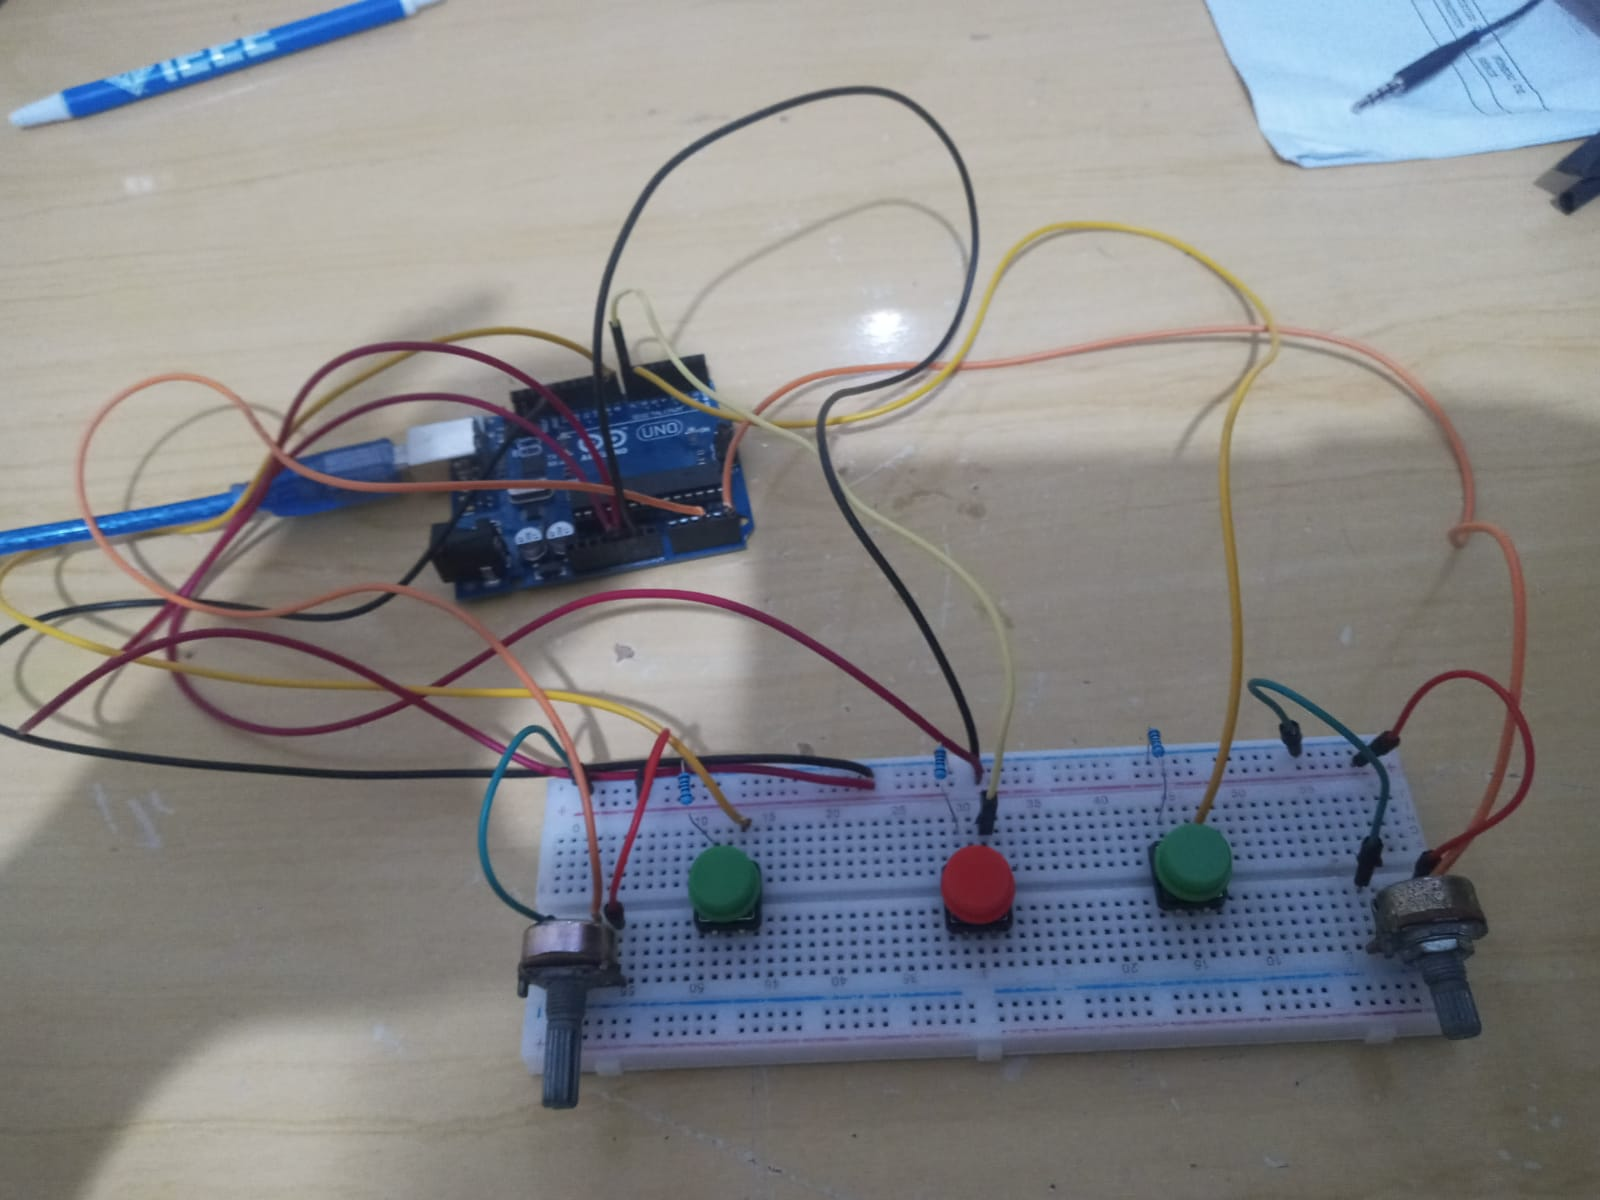
\includegraphics[width=0.6\textwidth]{circuito}
			\end{figure}
		\end{column}
			% Column 2    
			\begin{column}{0.7\textwidth}
				\begin{figure}
					\centering
						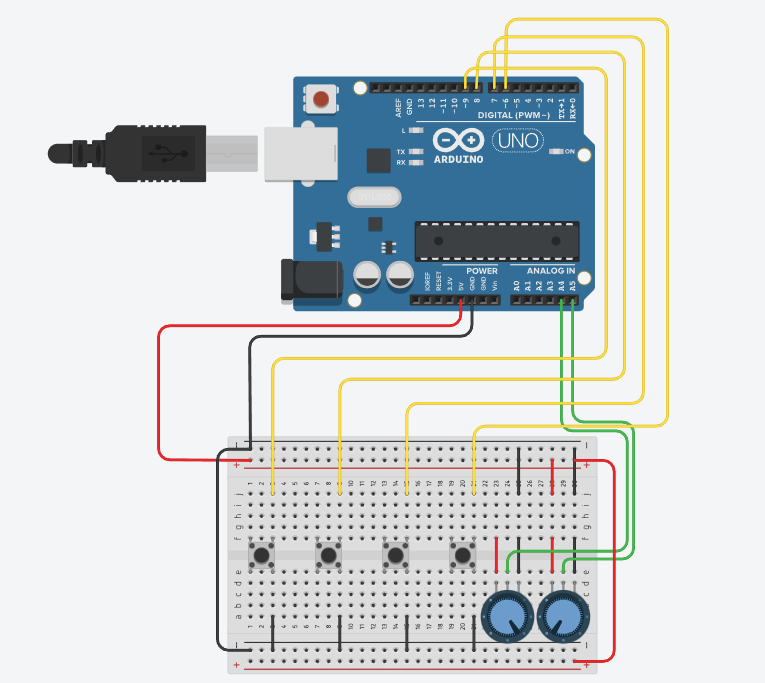
\includegraphics[width=0.4\textwidth]{esquematico-arduino}
				\end{figure}
			\end{column}
		\end{columns}

%*----------- notes
    \note[item]{Notes can help you to remember important information. Turn on the notes option.}
\end{frame}
%-
%*----------- SLIDE -------------------------------------------------------------
\begin{frame}[c]{Hardware - Controles}
 
  \begin{itemize}
      \item Modelos Impressos 3D para acomodar os botões e potenciômetros do circuito.
	\item Estes também são mais cômodos para os jogadores
    \end{itemize}
\vspace{0.3cm}
\begin{columns}
	% Column 1
	\begin{column}{0.4\textwidth}
		\begin{figure}
			\centering
    			\includegraphics[width=0.6\textwidth]{botão}
    			\caption{Os modelos impressos.}
    			%%\label{fig:question}
		\end{figure}
	\end{column}
		% Column 2    
		\begin{column}{0.4\textwidth}
			\begin{figure}
				\centering
    				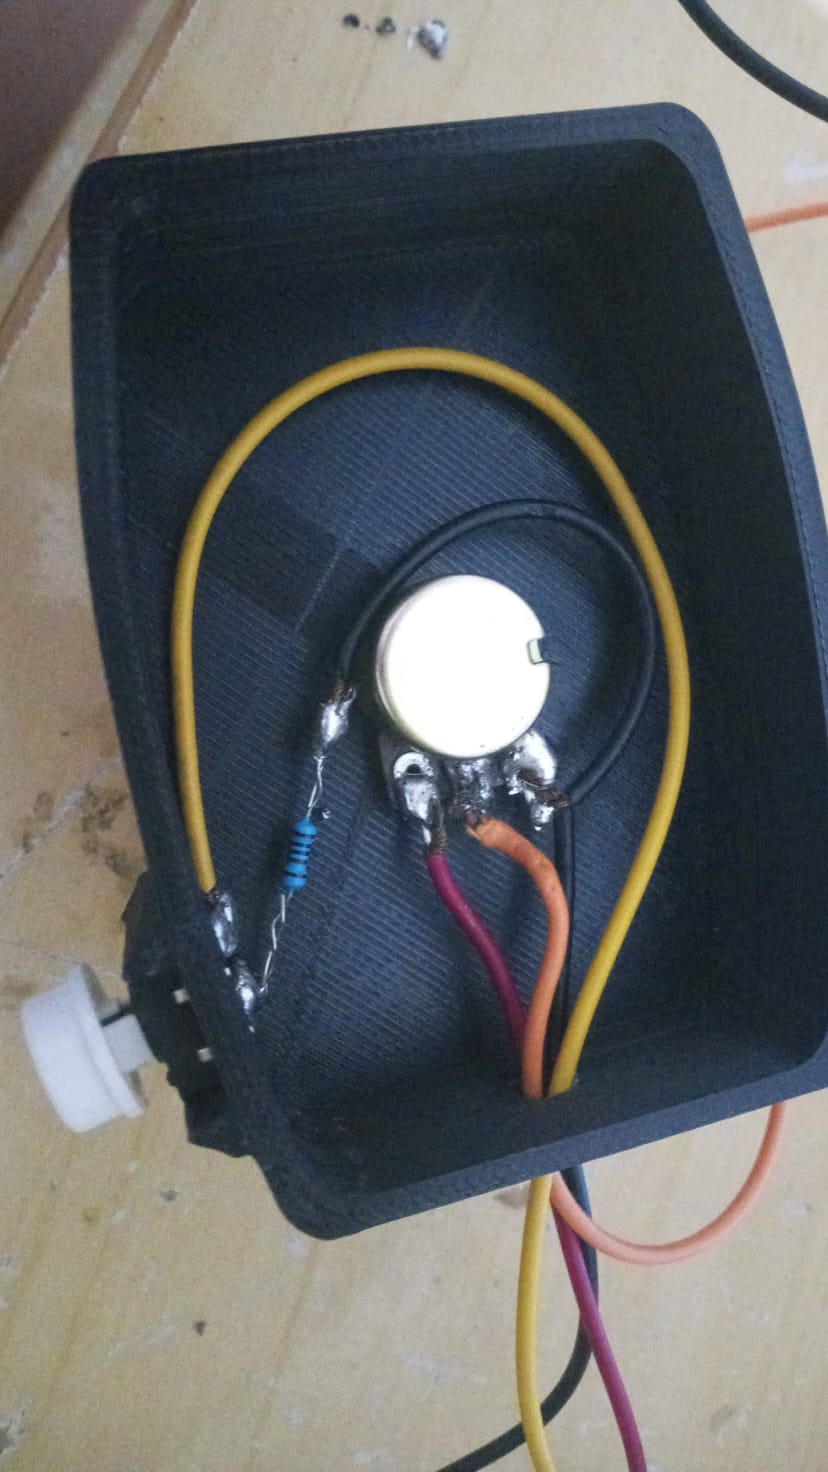
\includegraphics[width=0.4\textwidth]{solda}
    				\caption{A solda cos componentes no controle.}
    				%%\label{fig:question}
			\end{figure}
		\end{column}
	\end{columns}
%*----------- notes
    \note[item]{Notes can help you to remember important information. Turn on the notes option.}
 \end{frame}
%-
%*----------- SLIDE -------------------------------------------------------------
\begin{frame}[fragile]{Hardware - Arduino}
	 
\scriptsize
\begin{columns}
% Column 1
\begin{column}{0.5\textwidth}
	\begin{lstlisting}[language=C]
const int pot1 = A0, pot2 = A1; 
const int b01 = 8, b02 = 7; 
int v_pot1 = 0, v_pot2 = 0; 
bool v_b01,v_b02; 
int arr[10];

void setup() {
	Serial.begin(9600);
	pinMode(pot1, INPUT);
	pinMode(pot2, INPUT);
	for(int i = 7; i <= 8; i++){
	pinMode(i, INPUT_PULLUP);
	}
}
	\end{lstlisting}
\end{column}
% Column 2    
\begin{column}{0.55\textwidth}
	\begin{lstlisting}[language=C]
void loop() {

v_pot1 = map(analogRead(pot1),0,1023,0,255);
Serial.print(String(v_pot1) + "-");

v_pot2 = map(analogRead(pot2),0,1023,0,255);
Serial.print(String(v_pot2) + "-");

v_b01 = !digitalRead(b01);
v_b02 = !digitalRead(b02);

Serial.print(String(v_b01) + "-");
Serial.print(String(v_b02) + "\n");
delay(50);

}		
	\end{lstlisting}
\end{column}
\end{columns} 


%*----------- notes
    \note[item]{Notes can help you to remember important information. Turn on the notes option.}
 \end{frame}
%-
%*----------- SLIDE -------------------------------------------------------------
\begin{frame}[c]{Hardware - Arduino}
\vspace{0.2cm}
\begin{itemize}
        \item Como pode ser visto, uma string de modelo [x-x-x-x] é enviada ao Processing serialmente.
	  \item No Processing, essa string será separada em caracteres e cada um sera atribuido a sua respectiva classe.
    \end{itemize}

\begin{figure}
	\centering
    	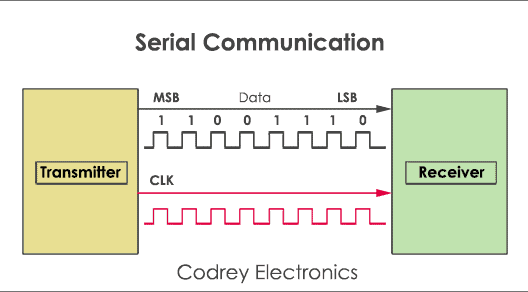
\includegraphics[width=0.4\textwidth]{serial}
    	%\caption{Representação d}
    	%%\label{fig:question}
\end{figure}

%*----------- notes
    \note[item]{Notes can help you to remember important information. Turn on the notes option.}
 \end{frame}
 %-
%*----------- SLIDE -------------------------------------------------------------
\begin{frame}
    

    
%*----------- notes
    \note[item]{Notes can help you to remember important information. Turn on the notes option.}
 \end{frame}
 %-
%*----------- SLIDE -------------------------------------------------------------
\begin{frame}
    %\transdissolve[duration=0.5]
    %\hspace*{-1cm}

  
 %*----------- notes__
    \note[item]{Notes can help you to remember important information. Turn on the notes option.}
\end{frame}
%-
%*----------- SLIDE -------------------------------------------------------------
\begin{frame}
    
  
 %*----------- notes__
    \note[item]{Notes can help you to remember important information. Turn on the notes option.}
\end{frame}
%-
%*----------- SLIDE -------------------------------------------------------------
\begin{frame}
    %\transdissolve[duration=0.5]
    
  
 %*----------- notes__
    \note[item]{Notes can help you to remember important information. Turn on the notes option.}
\end{frame}
%-
%*----------- SLIDE -------------------------------------------------------------
\begin{frame}
    %\transdissolve[duration=0.5]
    %\hspace*{-1cm}

  
 %*----------- notes
    \note[item]{Notes can help you to remember important information. Turn on the notes option.}
\end{frame}
 %-
%*----------- SLIDE -------------------------------------------------------------
\begin{frame}
    %\transdissolve[duration=0.5]
    %\hspace*{-1cm}
    
  
 %*----------- notes
    \note[item]{Notes can help you to remember important information. Turn on the notes option.}
\end{frame}
%-

